\documentclass[11pt,a4paper]{article}
\usepackage[a4paper,margin=2cm]{geometry}
\usepackage[]{graphicx}
\usepackage{bm}
\usepackage{apacite}
\bibliographystyle{apacite}
\usepackage{svg}
\usepackage{multirow}
\usepackage{amsmath}
\setlength{\parindent}{0pt}
\usepackage{pgf}
\usepackage{tikz}
\usepackage{pgfplots}
\usepackage{wrapfig}
\usepackage{float}
\usepackage[autostyle, english = american]{csquotes}
\usepackage[toc,page]{appendix}
\usepackage{amssymb}
\MakeOuterQuote{"}
\usepackage[T1]{fontenc}
\usepackage{enumitem}

\renewcommand{\baselinestretch}{1.1}
\setlist[enumerate]{itemsep=0mm}
\setlist[itemize]{itemsep=0mm}
\begin{document}
	\nocite{*}
	
	\begin{titlepage}
		
		
		\title{Determining the effect of electrolyte concentration of the voltage produced by galvanic cells}
		
		\author{Noah Alexiou}
		
		
		\date{June 2025}
		
		\maketitle
		\centering
		
	\end{titlepage}
	\tableofcontents
	\newpage
	
	
	\section{Rationale}
	
	
	\subsection{Background}

	

	\textbf{Redox}
	
	Redox reactions are reactions that involve the transfer of electrons between atoms. These reactions commonly occur within galvanic cells, which within themselves contain two half cells. 
	

	\textbf{Half Cells}
	
	Half cells consists of an electrolyte solution and electrode. When two are connected through a load and a salt  bridge, one of these half cells will become the anode, where oxidation occurs, and the other will become the cathode, where reduction occurs.
	
	The oxidised cell will transfer its electrons across a wire, where they will then reach and be accepted by the reduced cell.
	
	Each cell has its own standard electrode potential ($E^0$) which dictates the magnitude of electron emission, or attraction it has under standard lab conditions. 
	
	By measuring the difference in magnitude between cells, the overall potential between the cells can be quantified. 
	
	$$
	E^0_{\textrm{ Cell}}=E^0_{\textrm{ Cathode}}-E^0_{\textrm{ Anode}}
	$$
	What is the result of this?
	
	Why does this happen


\section{Methodology}
\subsection{Modifications}
\textbf{Half Cell Compositions}\newline
The results of original experiment indicated that copper and aluminum prodiced the largest voltage. It was theorized that after multiple trials, the aluminum would oxidise, skewing results.

It was decided that copper and zinc would be more suitable as alhough they produced a smaller voltage, zinc would take longer to oxidise and therefore produide more consistient results.

\textbf{Electrodes}\newline
Rather than thin strips, larger plates were bent into a "C" shape, slightly smaller than the diameter of the beaker they would be placed in. This maximised the sufrace area in contact with the electrolyte solution. Furthermore by resung the same electrodes, this sufrace area was constant for all trials.

\textbf{Measurement devices}\newline
A digiral multimeter was utlized to improve accuracy and extend the life of cells. This 

The original method is attached as an appendix
\subsection{Method}
\textbf{Materials}
\begin{itemize}
	\item 30ml $CuSO_4$ at concentrations $1.00\textrm{M}, 0.85\textrm{M}, 0.70\textrm{M}, 0.55\textrm{M}, 0.40\textrm{M}, 0.30\textrm{M}, 0.20\textrm{M}, 0.10\textrm{M}$
	\item 240ml $1$M$\;ZnSO_4$
	\item 20ml $KNO_3$
	\item Petri dish
	\item $50\textrm{ml}$ Beaker - x$2$
	\item zinc sheet $\approx4\textrm{cm}\times6\textrm{cm}$ 
	\item copper sheet $\approx4\textrm{cm}\times6\textrm{cm}$ 
	\item Emery paper
	\item Filter paper strips $\approx 2\textrm{cm}\times10\textrm{cm}$
	\item Digital Multimeter
	\item Alligator clips
	\item 150ml Plastic bottle - x16
	\item Tweezers 
	\item 1L Distilled water
	\item Emery paper
\end{itemize}

\textbf{Procedure}
\begin{enumerate}
	\item Pour varying amounts of $CUSO_4$ into 150ml plastic bottles and dilute with distilled water to form solutions with concentrations $1.00\textrm{M}, 0.85\textrm{M}, 0.70\textrm{M}, 0.55\textrm{M}, 0.40\textrm{M}, 0.30\textrm{M}, 0.20\textrm{M and } 0.10\textrm{M}$.
	
	\item Fill 8 of the 150ml plastic bottles with 30ml of 1M $ZnSO_4$ and set aside with copper solutions. 

	
	\item Polish electrodes with emery paper until they are shiny on all surfaces and then connect to alligator clips.
	
	\item Connect alligator clips to multimeter and set to DC voltage mode.
	
	\item Transfer the contents of a $CUSO_4$, and $ZnSO_4$ container into separate beakers.
	
	\item Wet salt bridge with $KNO_3$ and rest over the lip of both beakers, so that it is partially submerged in both. 
	
	\item Add the electrodes to the solution and record result as soon as value settles.
	
	\item Remove electrodes immediately and wash with distilled water. Stir electrolyte solutions with a glass stir rod. Remove salt bridge and dispose.
	
	\item Reconstruct cell with a new salt bridge, add electrodes back, and repeat measurementation so that there are three trials in total for any given concentration.
	
	\item Safely dispose of electrolyte solutions, wash equipment, and repeat for next $CUSO_4$ concentration.
\end{enumerate}

\subsection{Risk assessment}
Insert risk assessment

\section{Results}


\begin{figure}[h]
	\centering
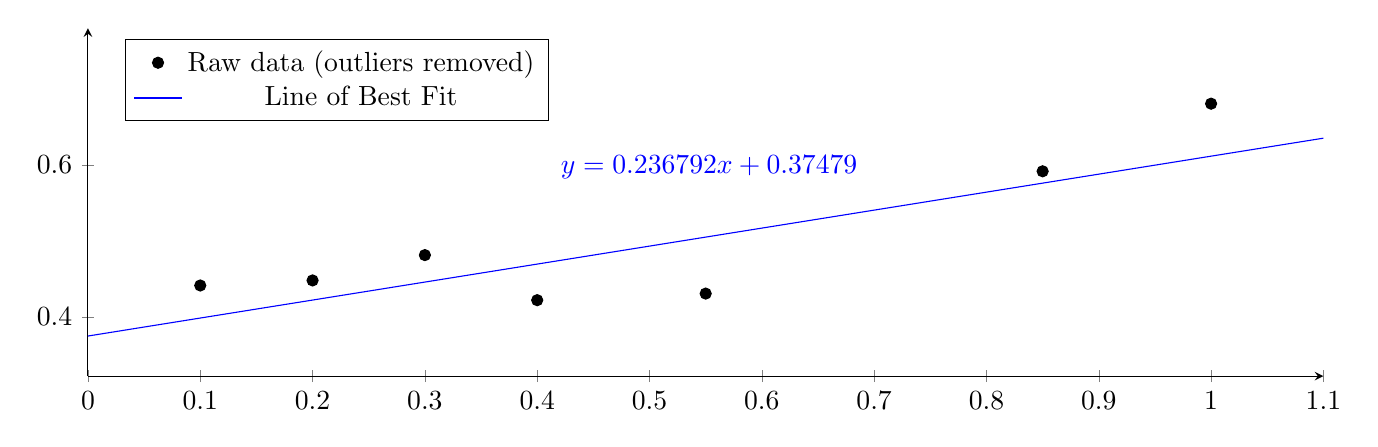
\begin{tikzpicture}
	\begin{axis}[xmin=0, xmax=1.1, ymin=0.322, ymax=0.78, axis lines=left, scale mode=stretch to fill, width=0.8\paperwidth, height=6cm, xtick distance=0.1, ytick distance=0.2, legend pos=north west]
		\addplot[only marks, mark=*, color=black]
		coordinates {
			(1, 0.680666666666667)
			(0.85, 0.591666666666667)
			(0.55, 0.430666666666667)
			(0.4, 0.422)
			(0.3, 0.481333333333333)
			(0.2, 0.448)
			(0.1, 0.441333333333333)
		};
		\addplot[no markers, blue, domain=0:1.1, samples=2, xlabel=] {(0.236792*x) + 0.37479};
	\node [anchor=south west,inner ysep=2.5cm, inner xsep=6cm, color=blue] {$y=0.236792x+0.37479$};
	\legend{Raw data (outliers removed), Line of Best Fit}
	\end{axis}
\end{tikzpicture}
\caption{Raw results with outliers removed with line of best fit.}
\end{figure}

\begin{figure}[h]
	\centering
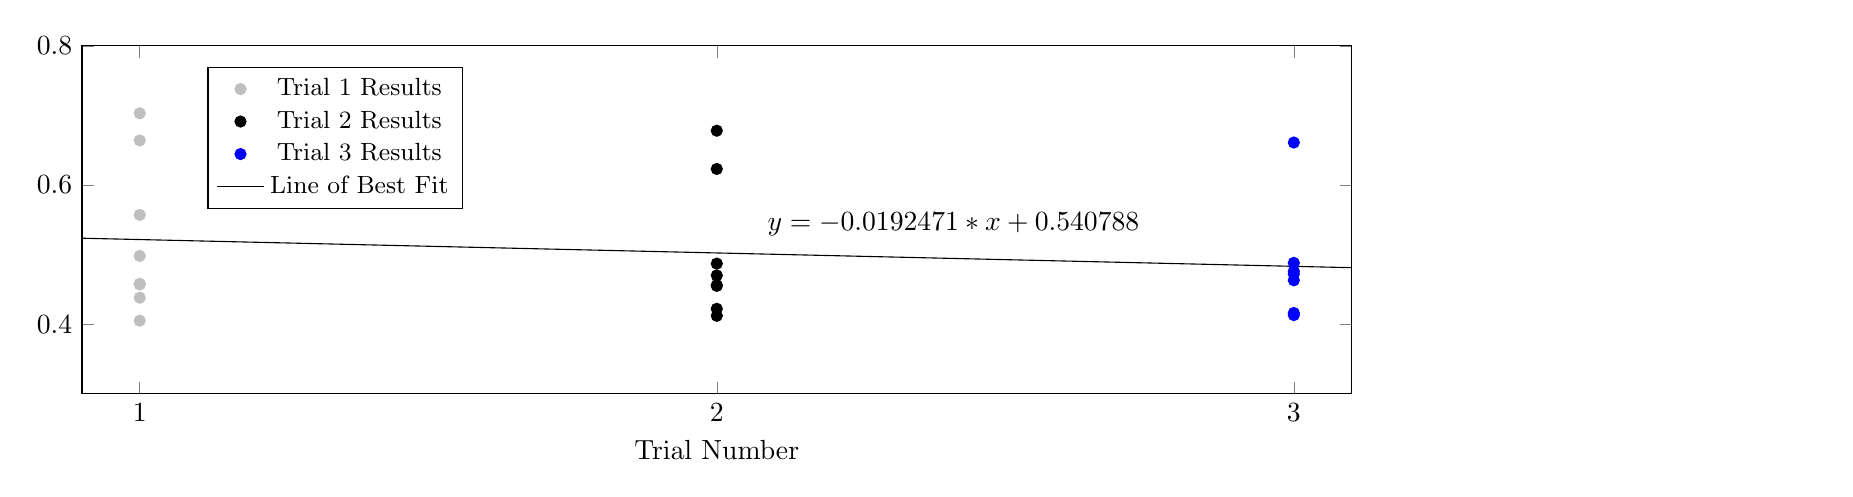
\begin{tikzpicture}
	\centering
	\begin{axis}[xmax=3.1, xmin=0.9, ymax=0.8, ymin=0.3, width=0.82\paperwidth, scale mode=stretch to fill, height=6cm, axis lines=box, clip=false, legend style={font=\small}, legend style={at={(0.3, 0.94)}},  xtick distance=1, xlabel={Trial Number}]
		\addplot [only marks, color=lightgray]
		coordinates{
		(1, 0.703)
		(1, 0.664)
		(1, 0.557)
		(1, 0.457)
		(1, 0.438)
		(1, 0.498)
		(1, 0.458)
		(1, 0.405)
	};

		\addplot [only marks, color=black]
		coordinates{
		(2, 0.678)
		(2, 0.623)
		(2, 0.455)
		(2, 0.422)
		(2, 0.412)
		(2, 0.47)
		(2, 0.487)
		(2, 0.456)
	};

		\addplot [only marks, color=blue]
		coordinates{
		(3, 0.661)
		(3, 0.488)
		(3, 0.472)
		(3, 0.413)
		(3, 0.416)
		(3, 0.476)
		(3, 0.463)		
		};
		\addplot [no markers, domain=0.9:3.1]{
		-0.0192471*x+0.540788
		};

		\node[anchor=south west, inner ysep=2cm, inner xsep=8.7cm]{$y=-0.0192471*x+0.540788$};
		
			\legend{Trial 1 Results, Trial 2 Results, Trial 3 Results, Line of Best Fit};
	\end{axis}
\end{tikzpicture}
\caption{Line of best fit for voltage over sequential trials}
\end{figure}



\end{document}